\section{Durchführung}
\label{sec:Durchführung}
\subsection{Aufbau}

In \autoref{fig:aufbau} ist der schematische Aufbau der genutzten Messapparatur dargestellt. 
\begin{figure}[H]
\centering
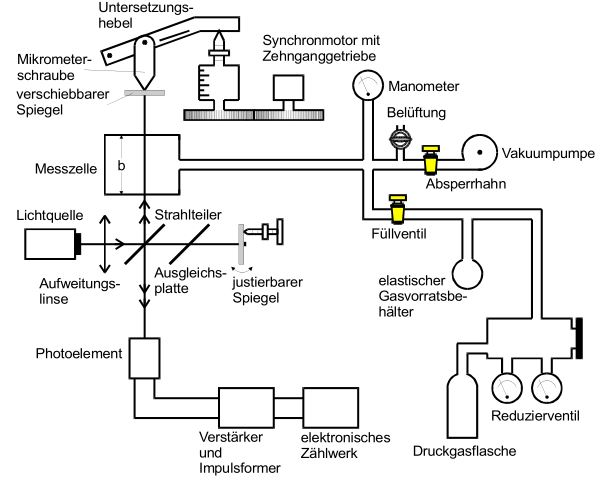
\includegraphics[width=\textwidth]{graphics/aufbau.JPG}
\caption{Schematischer Aufbau der genutzten Messapparatur. \cite{anleitung}}
\label{fig:aufbau}
\end{figure}

\subsection{Messvorgang}
Messapparatur kalibriert, einzelne Streifen übereinander

8 messreihen aufgenommen, Motor abwechselnd vor und zurück laufen gelassen
bei Geschwindigkeit 1, jeweils 5 mm range abgelesen an der
mikrometerschraube

Gleiche messweise diesmal mit druckänderung verursacht durch vakuumpumpe.
16 Messwerte 8 mal aufgepumpt 8 mal rausgelassen dabei drauf achten dass
die Änderung nicht zu schnell ist damit die richtige pulszahl gemessen
wird.
Übersetzung Wellenlänge
